\chapter{Symmetrien der Geradenkonfiguration} \label{chap:configsymm}
\section{Lineare und Kombinatorische Symmetrien}
Die Fermat-Flächen haben einen hohen Grad an Symmetrie. Offenbar lassen sowohl Permutationen der Koordinaten als auch Multiplikation der Koordinaten mit $d$-ten Einheitswurzeln die Fläche invariant. Damit operieren die Gruppen $S_4$ und $\mu_d^4$, letztere mit Stabilisator \note Heißt das so? isomorph zu $\mu_d$. Beide Gruppen schneiden sich nur in $\{\id\}$, also haben wir eine Aktion von
\begin{equation}
S_4 \ltimes \mu_d^4 / \mu_d \subset \PGL 4K,
\end{equation}
auf $F_d$, wobei der Homomorphismus $S_4 \rightarrow \Aut(\mu_d^4 / \mu_d)$ auf Permutationen der Koordinaten abbildet. In bestimmten Fällen gibt es sogar noch mehr Symmetrien, wie wir später sehen werden. Allgemein interessieren wir uns für Abbildungen aus~$\PGL 4K$ bzw.~$\PGaL 4K$, die die Fläche $F_d$ invariant lassen.\footnote{Für eine Theorie der linearen Gruppen, speziell der $\PGaL nK$, siehe \cite{Dieudonne}.}
\begin{defin}
Sei $S \in \proj n(K)$ eine beliebige Menge. Als lineare Symmetriegruppe von $S$ bezeichnen wir die Untergruppe
\begin{equation}
G_l = G_l(S) = \{ g \in \PGL{n+1}K: gS = S \}.
\end{equation}
\end{defin}

Solche linearen Abbildungen lassen nicht nur die Fläche invariant, sondern schicken auch Geraden auf Geraden. Damit permutieren sie die Geraden auf der Fläche, offenbar bleibt dabei aber ihre Schnittkonfiguration erhalten. Die Schnittkonfiguration wird durch einen Graphen $\mathcal G = (L,E)$ kodiert, dabei ist die $L$ die Menge der Geraden, und $(l_1, l_2) \in E$, wenn $l_1$ und $l_2$ sich schneiden.

Die Frage liegt nahe, welche Permutationen der Geraden es denn gibt, die die Schnittkonfiguration erhalten.
\begin{defin}
Sei nun $S \in \proj 3(K)$ eine projektive Fläche, $\mathcal G = (L,E)$ die Geradenkonfiguration. Dann ist die kombinatorische Symmetriegruppe von $S$ die Automorphismengruppe des Graphen $\mathcal G$, d.h.
\begin{equation}
G_k = G_k(S) = \{ \sigma \in \Sym(L): (l_1, l_2) \in E \Leftrightarrow (\sigma(l_1), \sigma(l_2)) \in E \}
\end{equation}
\end{defin}
Wir wollen in diesem Kapitel die Beziehung zwischen diesen beiden Gruppen ausarbeiten. Die folgende Betrachtung ist inspiriert durch \cite[Bem.~4.10.1, S.~404]{Hartshorne}, und \cite[Aufg. C--D, S.~180]{Mumford}. Dort wird die Situation für allgemeine reguläre Flächen dritten Grades untersucht.

Wie oben bemerkt, induziert jede lineare Symmetrie eine kombinatorische, also haben wir einen Homomorphismus $G_l(F_d) \to G_k(F_d)$.
\begin{prop}
Gibt es unter den Schnittpunkten der Geraden auf $S$ mindestens fünf in allgemeiner Lage,\footnote{das heißt: keine vier davon liegen auf einer projektiven Ebene.} so ist der Homomorphismus $G_l(S) \to G_k(S)$ injektiv.
\end{prop}
\begin{proof}
Sei $g \in \PGL 4K$ so gewählt, dass alle Geraden auf $S$ auf sich selbst abgebildet werden. Dann werden auch vier der Schnittpunkte auf sich selbst abgebildet. Sei $A \in \GL 4K$ ein Urbild von $g$, dann lässt also $A$ vier linear unabhängige eindimensionale Teilräume in $K^4$ invariant. Folglich hat $A$ in einer geeigneten Basis ${v_1, \dots v_4}$ des $K^4$ als Matrix Diagonalgestalt.

Sei $v_5 \in K^4 \setminus 0$ ein zugehöriger Vektor zum fünften Schnittpunkt. In der Basis $\{v_i\}_{i<5}$ hat $v_5$ dann die Gestalt $\sum_i \alpha_i v_i$ mit $\alpha_i \neq 0$ für alle $i$, da die fünf Schnittpunkte in allgemeiner Lage sind. Weil der fünfte Punkt von $g$ auf sich selbst geschickt wird, ist $A v_5 = \lambda v_5$ für ein $\lambda \in K^*$. Damit sind die Diagonaleinträge der Matrix alle gleich $\lambda$, da die $\alpha_i$ nicht verschwinden. Also ist $A = \lambda \id$ bzw.~$g = \id$.
\end{proof}
Wie wir weiter unten sehen werden, schneiden sich zwei Geraden einer Klasse in Punkten der Form $(1:\zeta^n:0:0)$, $\zeta \in \mu_{2d}$ primitiv und $n$ ungerade; sowie Permutationen der Koordinaten. Durch Probieren findet man damit leicht fünf Punkte in allgemeiner Lage. Die fünf $4 \times 4$-Untermatrizen von
\begin{equation*}
\begin{pmatrix}
1 & 0 & 1 & 0 & 1 \\
\zeta & 0 & 0 & 1 & 0 \\
0 & 1 & \zeta^3 & 0 & 0 \\
0 & \zeta & 0 & \zeta^5 & \zeta^3 \\
\end{pmatrix}
\end{equation*}
haben Determinanten $(\zeta^2-1)\zeta^4$, $(\zeta+1)\zeta^4$, $-(\zeta^3+1)\zeta^3$, $-(\zeta^3+1)\zeta^6$ bzw.~$(\zeta+1)\zeta^3$. Für $d>3$ verschwindet keine davon.

\section{Reguläre Geraden}
\paragraph{Konfiguration} Wir schreiben die Geraden aus \eqref{eq:regular} mit einer fixierten primitiven Einheitswurzel $\zeta \in \mu_{2d}$ und $a,b \in (2\mathbb Z + 1)/2d\mathbb Z \subset \Zmod 2dZ$:
\begin{equation}
\begin{split}
\Lcl(I)_{a,b}  :\qquad	&\langle (1,\zeta^a,0,0), (0,0,1,\zeta^b)\rangle \\
\Lcl(II)_{a,b} :\qquad	&\langle (1,0,\zeta^a,0), (0,1,0,\zeta^b)\rangle \\
\Lcl(III)_{a,b}:\qquad	&\langle (1,0,0,\zeta^a), (0,1,\zeta^b,0)\rangle.
\end{split}
\end{equation}
Ob sich zwei verschiedene projektive Geraden schneiden, stellt man anhand der Determinante der Matrix aus ihren vier Basisvektoren fest: verschwindet sie, dann hat die Matrix nicht vollen Rang, also schneiden sie sich in einem projektiven Punkt.

Damit überlegt man sich leicht, dass sich zwei Geraden aus derselben Familie genau dann schneiden, wenn sie in einem der beiden Parameter $a$, $b$ übereinstimmen. Für Geraden aus verschiedenen Klassen ergibt sich folgendes: zwei Geraden $\Lcl(I)_{a,b}$ und $\Lcl(II)_{a',b'}$ schneiden sich, wenn
\begin{equation}
\det \begin{pmatrix}
1 & \zeta^a & 0 & 0 \\
0 & 0 & 1 & \zeta^b \\
1 & 0 & \zeta^{a'} & 0 \\
0 & 1 & 0 & \zeta^{b'}
\end{pmatrix} = 0 \quad\Longleftrightarrow\quad \zeta^{a'} \zeta^b = \zeta^a \zeta^{b'} \quad\Leftrightarrow\quad a-b \equiv a'-b' \pmod{2d}.
\end{equation}
Analog erhält man, dass sich $\Lcl(I)_{a,b}$ und $\Lcl(III)_{a'',b''}$ schneiden, wenn $a''-b'' \equiv a+b$, und $\Lcl(II)_{a',b'}$ und $\Lcl(III)_{a'',b''}$, wenn $a''+b'' \equiv a'+b' \pmod{2d}$. \note Muss man das nachrechnen?

Die Schnittkonfiguration kann man sich also wie folgt vorstellen: Die Geraden teilen sich in drei Klassen, jede aus jeweils $d \times d$ Geraden bestehend. Ordnen wir die entsprechend in einer Matrix an, so schneiden sich alle Geraden in einer Zeile oder Spalte, die Zeilen und Spalten bilden also vollständige Graphen $K_d$. Zwischen den verschiedenen Klassen gibt es auch Schnitte: die Diagonalen verschiedener Klassen bilden einen bipartiten Graphen $K_{d,d}$. In der folgenden Grafik sind einige dieser Diagonalen dargestellt. Jede Gerade in einer der Diagonalen schneidet jede andere in der Diagonalen gleicher Farbe in der entsprechenden anderen Klasse. \note Ist das hilfreich?

\begin{figure}[h]
\centering
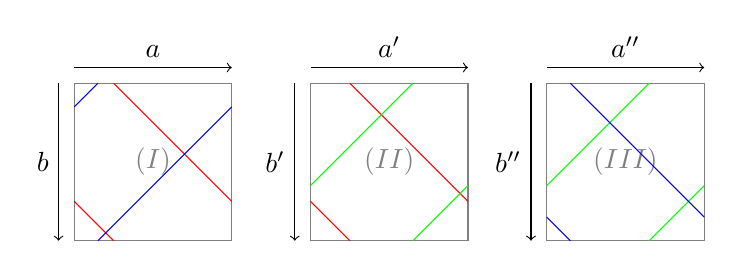
\begin{tikzpicture}
\draw[color=gray]
	[xshift=0cm] (0,0) rectangle (2,2) (1,1) node{$\Lcl(I)$}
	[xshift=3cm] (0,0) rectangle (2,2) (1,1) node{$\Lcl(II)$}
	[xshift=3cm] (0,0) rectangle (2,2) (1,1) node{$\Lcl(III)$};
\draw[->,xshift=0cm] (0,2.2) -- (2,2.2) node[above,midway] {$a$};
\draw[->,xshift=0cm] (-0.2,2) -- (-0.2,0)  node[left,midway] {$b$};
\draw[->,xshift=3cm] (0,2.2) -- (2,2.2) node[above,midway] {$a'$};
\draw[->,xshift=3cm] (-0.2,2) -- (-0.2,0)  node[left,midway] {$b'$};
\draw[->,xshift=6cm] (0,2.2) -- (2,2.2) node[above,midway] {$a''$};
\draw[->,xshift=6cm] (-0.2,2) -- (-0.2,0)  node[left,midway] {$b''$};
\draw[color=red]
	[xshift=0cm] (0.5,0) -- (0,0.5) (0.5,2) -- (2,0.5)
	[xshift=3cm] (0.5,0) -- (0,0.5) (0.5,2) -- (2,0.5);
\draw[color=green]
	[xshift=3cm] (1.3,0) -- (2,0.7) (0,0.7) -- (1.3,2)
	[xshift=3cm] (1.3,0) -- (2,0.7) (0,0.7) -- (1.3,2);
\draw[color=blue]
	[xshift=0cm] (0,1.7) -- (0.3,2) (0.3,0) -- (2,1.7)
	[xshift=6cm,yscale=-1,yshift=-2cm]
		(0,1.7) -- (0.3,2) (0.3,0) -- (2,1.7);
\end{tikzpicture}
\caption{Schnitte zwischen verschiedenen Klassen der regulären Geraden}\label{fig:reg}
\end{figure}

\paragraph{Symmetrien} Wir haben uns bereits klargemacht, dass wir auf $F_d$ eine Aktion der Gruppe $S_4 \ltimes \mu_d^4 / \mu_d$ haben, die nach obiger Proposition auch auf der Geradenkonfiguration transitiv operiert. Machen wir uns zunächst klar, auf welche Weise das geschieht. Multiplikation der $i$-ten Koordinate mit $\zeta^{s_i}$, $s_i$ gerade, bewirkt offenbar eine Verschiebung der Konfiguration in den einzelnen Klassen, und zwar wie folgt:

\begin{figure}[h]
\centering
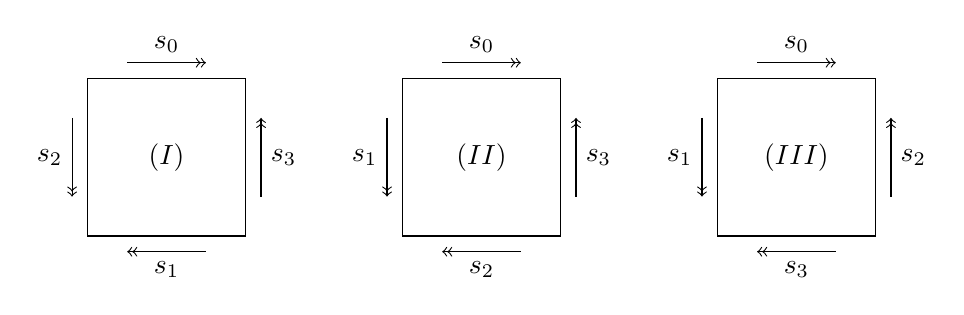
\begin{tikzpicture}
\draw[color=black]
	[xshift=0cm] (0,0) rectangle (2,2) (1,1) node{$\Lcl(I)$}
	[xshift=4cm] (0,0) rectangle (2,2) (1,1) node{$\Lcl(II)$}
	[xshift=4cm] (0,0) rectangle (2,2) (1,1) node{$\Lcl(III)$};
\draw[->>,xshift=0cm] (0.5,2.2) -- (1.5,2.2) node[above,midway] {$s_0$};
\draw[->>,xshift=0cm] (-0.2,1.5) -- (-0.2,0.5) node[left,midway] {$s_2$};
\draw[->>,xshift=0cm] (1.5,-0.2) -- (0.5,-0.2) node[below,midway] {$s_1$};
\draw[->>,xshift=0cm] (2.2,0.5) -- (2.2,1.5) node[right,midway] {$s_3$};

\draw[->>,xshift=4cm] (0.5,2.2) -- (1.5,2.2) node[above,midway] {$s_0$};
\draw[->>,xshift=4cm] (-0.2,1.5) -- (-0.2,0.5) node[left,midway] {$s_1$};
\draw[->>,xshift=4cm] (1.5,-0.2) -- (0.5,-0.2) node[below,midway] {$s_2$};
\draw[->>,xshift=4cm] (2.2,0.5) -- (2.2,1.5) node[right,midway] {$s_3$};

\draw[->>,xshift=8cm] (0.5,2.2) -- (1.5,2.2) node[above,midway] {$s_0$};
\draw[->>,xshift=8cm] (-0.2,1.5) -- (-0.2,0.5) node[left,midway] {$s_1$};
\draw[->>,xshift=8cm] (1.5,-0.2) -- (0.5,-0.2) node[below,midway] {$s_3$};
\draw[->>,xshift=8cm] (2.2,0.5) -- (2.2,1.5) node[right,midway] {$s_2$};
\end{tikzpicture}
\caption{Aktion von $\mu_d^4 / \mu_d$ auf der Geradenkonfiguration}\label{fig:coordmult}
\end{figure}

Die Aktion der Koordinatenpermutation ist schwieriger zu beschreiben. Man kann die drei Matrizen wie folgt auf einen Würfel kleben:

\begin{figure}[h] % we might need transform canvas={...} or sloping and slanting node text (http://tex.stackexchange.com/questions/62038/text-placed-in-pespective-on-3d-object)
\centering
\begin{tikzpicture}[x  = {(0.9659cm,0.25882cm)},
                    y  = {(-0.5cm,0.5cm)},
                    z  = {(0cm,1cm)}, scale = 2]
\begin{scope}[canvas is yx plane at z=0]
  \path[draw=black] (0,0) rectangle (2,2);
\end{scope}
\begin{scope}[canvas is zx plane at y=0]
  \path[draw=black] (0,0) rectangle (2,2);
\end{scope}
\begin{scope}[canvas is zy plane at x=0]
  \path[draw=black] (0,0) rectangle (2,2);
\end{scope}
\begin{scope}[canvas is yx plane at z=2]
  \path[draw=black] (0,0) rectangle (2,2);
\end{scope}
\begin{scope}[canvas is zx plane at y=2]
  \path[draw=black] (0,0) rectangle (2,2);
\end{scope}
\begin{scope}[canvas is zy plane at x=2]
  \path[draw=black] (0,0) rectangle (2,2);
\end{scope}
\end{tikzpicture}
\caption{Visualisierung der Aktion von $S_4$ auf der Geradenkonfiguration}\label{fig:perm}
\end{figure}

Dann entspricht die Aktion der $S_4$ der Drehgruppe des Würfels. \todo Hier fehlt noch einiges.

\paragraph{Vergleich der Symmetriegruppen} Wir zeigen nun, dass diese Symmetrien der Geradenkonfiguration die einzigen sind, die das Schnittverhalten respektieren. Zunächst müssen wir die Konfiguration aber genauer untersuchen.

\begin{lemma}
Sei $d \geq 4$, dann sind die einzigen Subgraphen isomorph zu $K_d$ die aus den Geraden einer Klasse bestehenden, die in einem der beiden Parameter übereinstimmen.
\end{lemma}
\begin{remarks}
Für $d=3$ ist das nicht der Fall: die drei Schnittpunkte der Diagonalen in Abb.~\ref{fig:reg} bilden ebenfalls einen $K_3$. (Die Grafik ist hier etwas irreführend: die Diagonalen schneiden sich für ungerades $d$ nur genau einmal.) \note Das ist etwas vage. Weglassen?
\end{remarks}
\begin{proof}
Sei $l \in L$ eine beliebige Gerade, dann schneidet sie jeweils $d-1$ Geraden in derselben Zeile bzw.~Spalte und jeweils $d$ Geraden in den entsprechenden Diagonalen in den anderen beiden Klassen. Wir wollen nun untersuchen, zu welchen vollständigen Graphen $K_d$ die Gerade $l$ gehört.

Von den $d$ Geraden in anderen Klassen, die $l$ schneiden, kann jeweils nur eine Teil des $K_d$ sein: denn diese schneiden sich untereinander nicht, da die Diagonalen von jeder Zeile und jeder Spalte jeweils nur eine Gerade beinhalten. Weiterhin gibt es keine Schnitte zwischen den Geraden in den anderen Klassen, die $l$ schneiden, und denen in derselben Klasse: denn die Geraden in den anderen Klassen schneiden die aus $l$'s Klasse genau dann, wenn sie in derselben Diagonale wie $l$ liegen. Die Diagonalen durch $l$ und die Zeile und Spalte von $l$ schneiden sich aber nur in $l$.

Da es zwischen den Geraden der Zeile von $l$ und der Spalte von $l$ keine weiteren Schnitte gibt, bleiben also drei Möglichkeiten für vollständige Graphen: die Geraden in der Zeile und Spalte von $l$ bilden jeweils einen $K_d$, und $l$ zusammen mit zwei ausgewählten Schnittpunkten in den anderen Klassen bildet einen $K_3$. Mehr ist aber nicht drin, und für $d \geq 4$ ist das nicht genug. Also sind sind alle auftretenden Subgraphen $K_d$ die Zeilen und Spalten einer Klasse.
\end{proof}
Das nächste Resultat besagt, dass kombinatorische Symmetrien die Partition in die Klassen respektieren.
\begin{lemma}
Sei $d \geq 4$, $\sigma \in G_k$ eine kombinatorische Symmetrie und $l_1, l_2 \in L$ zwei Geraden. Sind $l_1$ und $l_2$ in derselben Klasse, dann auch ihre Bilder $\sigma(l_1)$, $\sigma(l_2)$.
\end{lemma}
\begin{proof}
Das vorige Lemma besagt, dass alle vollständigen Subgraphen $K_d$ vollständig in einer Klasse enthalten sind. Gleichzeitig wissen wir, dass jede Gerade zu zwei solchen Subgraphen gehört. Damit ist dieses Lemma offensichtlich: man setze die symmetrische, reflexive Relation
\begin{equation*}
l_1 \sim l_2 \Longleftrightarrow l_1, l_2 \text{ gehören zu einem gemeinsamen Subgraphen } K_d
\end{equation*}
auf den Geraden transitiv fort, dann sind die Äquivalenzklassen genau die drei Klassen $\Lcl(I)$, $\Lcl(II)$, $\Lcl(III)$. Weil die Relation sich offenbar mit Symmetrien verträgt, bleiben also die drei Klassen invariant.
\end{proof}

Damit haben wir einen Homomorphismus $G_k \to S_3$, der eine kombinatorische Symmetrie auf die entsprechende Permutation der Klassen schickt. Der Kern besteht dann aus denjenigen Symmetrien, die alle drei Klassen invariant lassen. Sei $\tilde{\mathcal G}$ der Graph einer Klasse, d.\,h.~einen Graphen $\mathcal G$ mit Knotenmenge $\{1,\dots,d\}^2$ und Kanten $(a,b) \sim (a',b') \Longleftrightarrow a=a' \vee b=b'$. Dann gilt offenbar
\begin{equation}
\ker(G_k \to S_3) \subseteq (\Aut \tilde{\mathcal G})^3.
\end{equation}
Daher liegt es nahe, zunächst $\Aut(\tilde{\mathcal G})$ zu untersuchen.

Offenbar können sowohl die Zeilen als auch die Spalten beliebig untereinander permutiert werden, und eine Vertauschung von Zeilen und Spalten (Transposition) ist auch möglich. Wir zeigen jetzt, dass mehr nicht geht.
\begin{lemma}
Betrachte den Subgraph $\tilde{\mathcal G}$ einer Klasse $\Lcl(I/II/III)$. Sei $\sigma \in \Aut \tilde{\mathcal G}$, dann bildet $\sigma$ entweder Zeilen auf Zeilen und Spalten auf Spalten ab, oder Zeilen auf Spalten und Spalten auf Zeilen.
\end{lemma}
\begin{proof}
Wir betrachten die Zeile $\{1,\dots,d\} \times \{1\}$, ihr Bild ist eine Zeile oder Spalte. Ohne Beschränkung der Allgemeinheit können wir annehmen, dass sie auf sich selbst abgebildet wird. (Sonst transponiere entsprechend und permutiere die Zeilen, das ändert nichts an der Aussage.)

Die Menge der Spalten ist nun $\{\{i\} \times \{1,\dots,d\} : 1 \leq i \leq d\}$. Die Knoten einer Spalte haben die Eigenschaft, dass sie alle mit einem und demselben Knoten in der Zeile $\{1,\dots,d\} \times \{1\}$ verbunden sind. Damit sind ihre Bilder alle mit einem und demselben Knoten im Bild der Zeile $\{1,\dots,d\} \times \{1\}$ verbunden. Folglich sind die Bilder der Spalten wieder Spalten. Damit werden aber auch die restlichen Zeilen auf Zeilen abgebildet. Was anderes bleibt ihnen ja nicht übrig, da es nur $2d$ vollständige Subgraphen $K_d$ in $\tilde{\mathcal G}$ gibt.
\end{proof}

Das liefert uns nun sogar einen Homomorphimus $\pi \colon G_k \to S_3 \ltimes_{\text{kan.}} C_2^3$, der eine kombinatorische Symmetrie auf die Permutation der Klassen und Transposition innerhalb der Klassen abbildet. Der Kern besteht nun aus Symmetrien, die alle Klassen invariant lassen und Zeilen auf Zeilen und Spalten auf Spalten schicken.

Damit bleibt nur eine Permutation der Zeilen bzw. Spalten, damit liegt der Kern in $(S_d \times S_d)^3$. Mit den Schnitten zwischen verschiedenen Klassen wollen wir das auf eine deutlich kleinere Gruppe einschränken.
\begin{prop}
Zwei Geraden einer Klasse liegen auf derselben Diagonale genau dann, wenn sie einander nicht schneiden, aber es mindestens $d$ Geraden gibt, die beide schneiden.
\end{prop}
\begin{proof}
Die eine Richtung ist klar. Seien nun zwei Geraden $l_1$, $l_2$ gegeben mit $l_1 \not\sim l_2$, sodass aber $d$ Geraden $k_1, \dots, k_d \in L$ existieren mit $l_1 \sim k_i \sim l_2$ für $1 \leq i \leq d$. Wegen $l_1 \not\sim l_2$ liegen beide nicht in derselben Zeile oder Spalte, also liegen auch die $k_i$ nicht in derselben Zeile oder Spalte, sie liegen also in anderen Klassen.

Die zu $l_1$, $l_2$ inzidenten Geraden in anderen Klassen liegen auf jeweils parallelen Diagonalen in diesen Klassen. Gemeinsame inzidente Geraden gibt es also nur dann, wenn entsprechende Diagonalen zusammenfallen. Damit liegen aber auch $l_1$, $l_2$ auf einer gemeinsamen Diagonale.
\end{proof}
\begin{coroll}
Damit bilden kombinatorische Symmetrien Diagonalen auf Diagonalen ab.
\end{coroll}
Nun zeigen wir noch, dass parallele Diagonalen auf parallele Diagonalen abgebildet werden. Das ist nicht so trivial, wie es klingt: transversale Diagonalen müssen sich für gerades $d$ nicht schneiden.
\begin{prop}
Eine Symmetrie $\sigma \in \ker \pi$ schickt Diagonalen in einer Klasse auf zu Ihnen parallele Diagonalen.
\end{prop}
\begin{proof}
Wegen Symmetrie der Klassen können wir annehmen, dass es sich um die rote Diagonale in Klasse $\Lcl(I)$ von Abb.~\ref{fig:reg}, d.\,h. eine Diagonale mit konstanter Differenz $a-b$ handelt. Die Geraden auf dieser Diagonale haben gemeinsame inzidente Geraden in $\Lcl(II)$. Da $\sigma$ die Klassen invariant lässt, gilt dies auch für das Bild der Diagonale. Also handelt es sich um eine zur roten parallelen Diagonale.
\end{proof}

\begin{lemma}
Ein Automorphismus des Graphen $\tilde{\mathcal G}$, der Diagonalen auf dazu parallele Diagonalen schickt, hat die Form $((2\mathbb Z+1)/2d\mathbb Z)^2 \to ((2\mathbb Z+1)/2d\mathbb Z)^2, (x,y) \mapsto (Cx+D_1, Cx+D_2)$ mit $C \in (\Zmod 2dZ)^*$, $D_1, D_2 \in 2\Zmod 2dZ$.
\end{lemma}
\begin{proof}
Sei also $(\sigma, \tau) \in S_d \times S_d$, $\{(a,b) : a-b \equiv c \pmod{2d}\}$ mit $c \in 2\Zmod 2dZ$ eine Diagonale. Dann soll auch ihr Bild eine Diagonale sein, d.\,h. $\sigma(a) - \tau(b) \equiv c' \pmod{2d}$ für alle $(a,b)$ mit $a-b \equiv c \pmod{2d}$. Damit ist $\tau(b) \equiv c' + \sigma(a) \equiv c' + \sigma(c+b)$, es ergibt sich also $\tau$ aus $\sigma$. Subtrahiert man die Gleichungen für $c_1=0$, $c_2=2$, so erhält man
\begin{equation*}
\sigma(b+2) - \sigma(b) \equiv c_2' - c_1' =: C \qquad\Longleftrightarrow\qquad \sigma(b+2) \equiv \sigma(b) + C  \mod{2d}.
\end{equation*}
Damit ist $\sigma$ offenbar von der Form $\sigma(x) = Cx+D_1$ und $\tau$ entsprechend von der Form $\tau(x) = c' + C(c+x) + D_1 = Cx + (c'+Cc+D_1) = Cx + D_2$, $D_2 := c'+Cc+D_1$.
\end{proof}

\begin{lemma}
Der Kern von $\pi \colon G_k \to S_3 \ltimes C_2^3$ besteht aus Verschiebungen der Parameter $a$, $b$ in den drei Klassen und Multiplikation aller Parameter mit einem Faktor aus $(\Zmod 2dZ)^*$. Genauer: es gibt eine Einbettung $\ker \pi \into (\Zmod 2dZ)^* \ltimes_\alpha (2\Zmod 2dZ)^6$, wobei $\alpha \colon (\Zmod 2dZ)^* \to \Aut((2\Zmod 2dZ)^6)$ durch koordinatenweise Multiplikation definiert ist.
\end{lemma}
\begin{proof}
Nach den vorigen beiden Aussagen ist nur noch zeigen, dass die Faktoren $C$ in allen drei Klassen gleich sein müssen. Das ist aber klar: zwei Diagonalen mit Abstand $2$ haben im Bild einen Abstand $2C$. Damit Geraden auf derselben Diagonalen inzident bleiben mit den entsprechenden Diagonalen in anderen Klassen, müssen offenbar die Faktoren $C$ übereinstimmen.
\end{proof}

Offenbar können wir also eine Symmetrie aus dem Kern $\sigma$ in zwei Teile zerlegen: eine Skalarmultiplikation aller Parameter mit $C \in (\Zmod 2dZ)^*$ und eine anschließende Verschiebung um eine Vektor $(\alpha_1, \beta_1, \dots, \alpha_3, \beta_3) \in (2\Zmod 2dZ)^6$. Diese ist aber nicht beliebig, vielmehr gelten folgende Relationen:
\begin{align*}
\text{rot:}\qquad  \alpha_1 - \beta_1 &= \alpha_2 - \beta_2 \\
\text{grün:}\qquad \alpha_2 + \beta_2 &= \alpha_3 + \beta_3 \\
\text{blau:}\qquad \alpha_1 + \beta_1 &= \alpha_3 - \beta_3
\end{align*}
Das ergibt sich aus den resultierenden Verschiebungen der Diagonalen, siehe Abb.~\ref{fig:reg}. Diese drei Gleichungen sind unabhängig, wie man sich leicht überzeugt. Der Lösungsraum ist isomorph zu $(2\Zmod 2dZ)^3 \cong (\Zmod dZ)^3 \cong C_d^3$.

Jetzt schränken wir noch das Bild von $G_k \to S_3 \ltimes C_2^3$ ein: hoffentlich ist es isomorph zu $S_4$. Offenbar hat $S_4$ Index $2$ in $S_3 \ltimes C_2^3$. Es reicht also zu zeigen, dass es eine Symmetrie aus $S_3 \ltimes C_2^3$ gibt, die das Schnittverhalten nicht erhält. \note Wie begründet man das?

Das Bild von $S_4$ unter $S_4 \into G_l \to G_k \to S_3 \ltimes C_2^3$ ist isomorph zu $S_4$: denn die Komposition ist injektiv, wie man sich schnell klar macht. Dass das Bild von $G_k \to S_3 \ltimes C_2^3$ nicht größer ist, folgt dann mit obigem Argument. Das ist aber tatsächlich nicht einfach...

\begin{theorem}
Sei $d \geq 4$ und $\Char K=0$, dann sind die einzigen Symmetrien der Geradenkonfiguration die durch die lineare Gruppe erzeugten.
\end{theorem}
\begin{proof}
Das sollte nun recht schnell mit obigem folgen.
\end{proof}

\section{Geistergeraden}
\paragraph{Konfiguration}
\paragraph{Symmetrien}
% Betrachtung der irregulären Situation